\chapter{\textbf{Estado da arte e base teórica}}

\section{Primeira secção}
%blindtext is used to generate a random text to show how text looks in the pdf
\Blindtext

%example for a figure, figures should be saved in the folder 'fig'
\begin{figure}[ht]
	\centering

		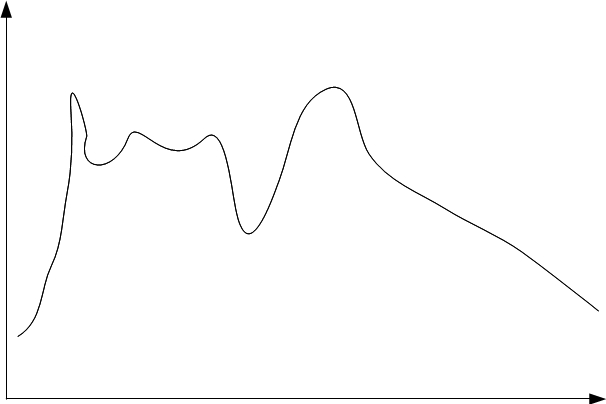
\includegraphics[width=0.8\textwidth]{pic/example.jpg}

	\caption[First example.]{First example to describe how short and long caption work for figures. Everything written in the square brackets will be listed in the list of figures, everything written in the curly brackets will be shown directly underneath the figure.}

	\label{fig:firstexample}
\end{figure}




%example for a crossreference (here: figure)
Here I will reference the first figure (see figure \ref{fig:firstexample}). Also, in \ref{res:subfigure} a figure with multiple subfigures is shown.

\noindent %no indent is generated in the new paragraph
The we can make a list of different things:

%example for a list without numbers
\begin{itemize} 
\item First item on the list
\item Second item on the list 
\item Third item on the list 
\end{itemize}


\section{Segunda secção}

Outro tipo de lista:

\begin{itemize}[noitemsep]
%\setlength\itemsep{1em}
\item[--] \textbf{Item 1:} Descrição do primeiro item;
\item[--] \textbf{Item 2:} Descrição do segundo item;
\item[--] \textbf{Item 4:} Descrição do terceiro item;
\item[--] \textbf{Item 5:} Descrição do quarto item;
\end{itemize}


\addtocontents{toc}{\vspace{0.8cm}} % -> add space in TOC 